\documentclass[aspectratio=169,10pt]{beamer}

% A self-contained Beamer presentation for a mathematical audience.
% Compile with: pdflatex informative_sampling_control_presentation.tex

\usepackage[T1]{fontenc}
\usepackage[utf8]{inputenc}
\usepackage{lmodern}
\usepackage{amsmath,amssymb,mathtools}
\usepackage{booktabs,array}
\usepackage{ragged2e}
\usepackage{tikz}
\usetikzlibrary{arrows.meta,calc,positioning,fit,backgrounds}
\usepackage{pgfplots}
\pgfplotsset{compat=1.18}

% ---------- Visual language ----------
\definecolor{Ink}{HTML}{102A43}
\definecolor{Teal}{HTML}{007C83}
\definecolor{Sky}{HTML}{E7F4F4}
\definecolor{Coral}{HTML}{E46C5B}
\definecolor{Gold}{HTML}{E8AE3A}
\definecolor{Slate}{HTML}{526777}
\definecolor{Mist}{HTML}{F4F7F9}
\definecolor{PaleGold}{HTML}{FFF5D9}

\setbeamercolor{normal text}{fg=Ink,bg=white}
\setbeamercolor{structure}{fg=Teal}
\setbeamercolor{frametitle}{fg=Ink,bg=white}
\setbeamercolor{title}{fg=white}
\setbeamercolor{subtitle}{fg=Sky}
\setbeamercolor{alerted text}{fg=Coral}
\setbeamercolor{block title}{fg=white,bg=Teal}
\setbeamercolor{block body}{fg=Ink,bg=Sky}
\setbeamercolor{itemize item}{fg=Teal}
\setbeamercolor{itemize subitem}{fg=Coral}

\setbeamertemplate{navigation symbols}{}
\setbeamertemplate{itemize item}{\raise0.2ex\hbox{\scriptsize$\blacktriangleright$}}
\setbeamertemplate{itemize subitem}{\raise0.15ex\hbox{\tiny$\bullet$}}
\setbeamertemplate{frametitle}{%
  \vspace{0.28cm}\hspace{0.15cm}\insertframetitle\par
  \vspace{-0.18cm}\hspace{0.15cm}{\color{Teal}\rule{1.35cm}{1.7pt}}\vspace{0.08cm}
}
\setbeamertemplate{footline}{%
  \leavevmode\hbox{%
  \begin{beamercolorbox}[wd=\paperwidth,ht=2.7ex,dp=1.15ex,leftskip=.55cm,rightskip=.55cm]{author in head/foot}%
    \color{Slate}\scriptsize Prior-informed data generation for learned controllers
    \hfill\color{Teal}\insertframenumber/\inserttotalframenumber
  \end{beamercolorbox}}
}

\setbeamersize{text margin left=0.65cm,text margin right=0.65cm}
\setlength{\parskip}{0.35em}

\newcommand{\R}{\mathbb{R}}
\newcommand{\Xf}{\mathcal{X}_{\mathrm{feas}}}
\newcommand{\D}{\mathcal{D}}
\newcommand{\risk}{\mathcal{R}_{\mathrm{cl}}}
\newcommand{\smallsource}[1]{\vfill\begin{flushleft}\color{Slate}\tiny #1\end{flushleft}}
\newcommand{\pill}[2]{\tikz[baseline=(X.base)]\node[rounded corners=2pt,fill=#1,inner xsep=5pt,inner ysep=2pt] (X) {\scriptsize\color{Ink}#2};}

\title{Prior-informed data generation\\for learned controllers}
\subtitle{How can mathematical structure buy sample efficiency?}
\author{Pietro Gori}
\institute{University of Pisa}
\date{October 2026}

\begin{document}

% -----------------------------------------------------------------------------
\begin{frame}[plain]
  \begin{tikzpicture}[remember picture,overlay]
    \fill[Ink] (current page.south west) rectangle (current page.north east);
    \fill[Teal] ([xshift=-4.0cm]current page.north east) -- (current page.north east) --
      (current page.south east) -- ([xshift=-7.1cm]current page.south east) -- cycle;
    \draw[white,opacity=.13,line width=0.6pt]
      ([xshift=-5.2cm,yshift=-1.0cm]current page.north east) circle (2.0cm);
    \draw[white,opacity=.13,line width=0.6pt]
      ([xshift=-2.3cm,yshift=-4.1cm]current page.north east) circle (2.8cm);
  \end{tikzpicture}
  \vspace{1.1cm}
  {\usebeamerfont{title}\color{white}\LARGE\bfseries\inserttitle\par}
  \vspace{0.35cm}
  {\color{Sky}\large\insertsubtitle\par}
  \vfill
  {\color{white}\normalsize\insertauthor\par}
  {\color{Sky}\small\insertinstitute\hfill\insertdate\par}
  \note{Open with the practical tension: optimization gives excellent controllers, but using them as teachers makes every label expensive. The talk asks how mathematics can decide which labels deserve to be computed.}
\end{frame}

% -----------------------------------------------------------------------------
\begin{frame}{The practical origin: an expensive teacher}
\begin{columns}[T,onlytextwidth]
  \column{0.56\textwidth}
  \textbf{Online goal.} Replace a constrained nonlinear or switched MPC policy by a fast neural policy
  \[
    \pi_\theta(x) \approx \pi^\star_{\mathrm{MPC}}(x).
  \]

  \textbf{Offline cost.} Each label requires an optimal-control solve
  \[
    x^{(i)} \longmapsto u^{\star(i)}_0,
    \qquad \D_N=\{(x^{(i)},u^{\star(i)}_0)\}_{i=1}^{N}.
  \]

  \textbf{Observed bottleneck.} Most solver calls confirm behavior already represented in the dataset, while rare states determine constraint violations or closed-loop failure.

  \column{0.40\textwidth}
  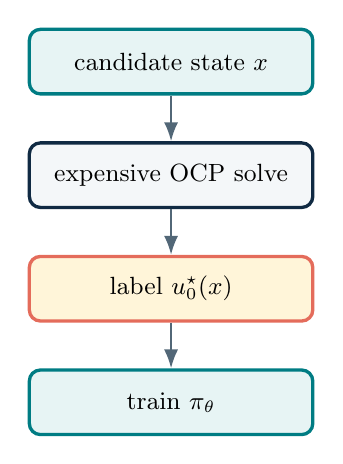
\begin{tikzpicture}[node distance=0.58cm, every node/.style={font=\small,align=center}]
    \node[draw=Teal,very thick,rounded corners,fill=Sky,minimum width=3.6cm,minimum height=.82cm] (x) {candidate state $x$};
    \node[draw=Ink,very thick,rounded corners,fill=Mist,below=of x,minimum width=3.6cm,minimum height=.82cm] (ocp) {expensive OCP solve};
    \node[draw=Coral,very thick,rounded corners,fill=PaleGold,below=of ocp,minimum width=3.6cm,minimum height=.82cm] (lab) {label $u_0^\star(x)$};
    \node[draw=Teal,very thick,rounded corners,fill=Sky,below=of lab,minimum width=3.6cm,minimum height=.82cm] (nn) {train $\pi_\theta$};
    \draw[-{Latex[length=2.4mm]},thick,Slate] (x)--(ocp);
    \draw[-{Latex[length=2.4mm]},thick,Slate] (ocp)--(lab);
    \draw[-{Latex[length=2.4mm]},thick,Slate] (lab)--(nn);
  \end{tikzpicture}
\end{columns}
\smallsource{Approximate MPC reduces online computation, but training-data generation can be prohibitively expensive: Krishnamoorthy, IEEE TAC, 2022.}
\note{Connect this directly to your own active-set and projection-based sampling work. Stress that the teacher is not a human annotator. It is an optimization problem whose structure is available.}
\end{frame}

% -----------------------------------------------------------------------------
\begin{frame}{Why random sampling misses what matters}
\begin{columns}[T,onlytextwidth]
\column{0.47\textwidth}
\centering
\textbf{Passive sampling}

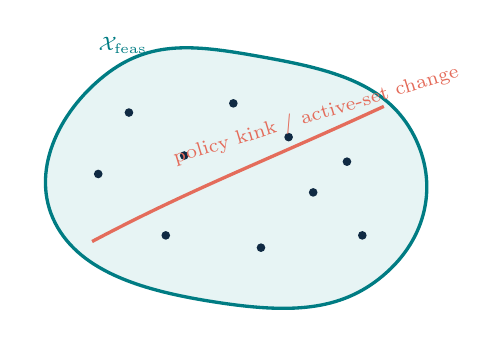
\begin{tikzpicture}[scale=.78]
  \fill[Sky] plot[smooth cycle,tension=.8] coordinates {(-3,-.7) (-2.2,1.7) (0.4,2.0) (2.8,.8) (2.4,-1.5) (-.3,-2.0)};
  \draw[Teal,very thick] plot[smooth cycle,tension=.8] coordinates {(-3,-.7) (-2.2,1.7) (0.4,2.0) (2.8,.8) (2.4,-1.5) (-.3,-2.0)};
  \draw[Coral,very thick] (-2.4,-1.0) .. controls (-.8,-.15) and (.4,.3) .. (2.35,1.2);
  \foreach \p in {(-2.3,.1),(-1.8,1.1),(-1.2,-.9),(-.9,.4),(-.1,1.25),(.35,-1.1),(.8,.7),(1.2,-.2),(1.75,.3),(2.0,-.9)}
    \fill[Ink] \p circle (2.0pt);
  \node[font=\scriptsize,Teal] at (-1.9,2.2) {$\Xf$};
  \node[font=\scriptsize,Coral,rotate=17] at (1.25,1.05) {policy kink / active-set change};
\end{tikzpicture}

Uniform coverage spends many labels in smooth interiors.

\column{0.47\textwidth}
\centering
\textbf{Structure-informed sampling}

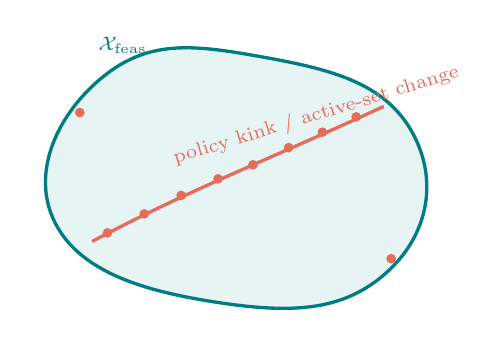
\begin{tikzpicture}[scale=.78]
  \fill[Sky] plot[smooth cycle,tension=.8] coordinates {(-3,-.7) (-2.2,1.7) (0.4,2.0) (2.8,.8) (2.4,-1.5) (-.3,-2.0)};
  \draw[Teal,very thick] plot[smooth cycle,tension=.8] coordinates {(-3,-.7) (-2.2,1.7) (0.4,2.0) (2.8,.8) (2.4,-1.5) (-.3,-2.0)};
  \draw[Coral,very thick] (-2.4,-1.0) .. controls (-.8,-.15) and (.4,.3) .. (2.35,1.2);
  \foreach \p in {(-2.15,-.86),(-1.55,-.55),(-.95,-.25),(-.35,.02),(.22,.25),(.8,.53),(1.35,.78),(1.9,1.03),(2.47,-1.28),(-2.6,1.1)}
    \fill[Coral] \p circle (2.25pt);
  \node[font=\scriptsize,Teal] at (-1.9,2.2) {$\Xf$};
  \node[font=\scriptsize,Coral,rotate=17] at (1.25,1.05) {policy kink / active-set change};
\end{tikzpicture}

Concentrate labels near changes, boundaries, and likely trajectories.
\end{columns}

\vspace{0.2cm}
\begin{center}
\colorbox{PaleGold}{\parbox{0.88\textwidth}{\centering\textbf{The design variable is the data distribution, not only the model architecture.}}}
\end{center}
\note{The red curve is schematic. For parametric programs, active-set changes often induce a piecewise-smooth policy. These regions can dominate approximation error even when they occupy little volume.}
\end{frame}

% -----------------------------------------------------------------------------
\begin{frame}{Mathematical statement}
For an initial state $x$, define the parametric optimal-control problem
\begin{align*}
  z^\star(x)\in\arg\min_z\quad & J(z;x) \\
  \text{s.t.}\quad & c(z;x)=0, \qquad g(z;x)\le 0,
\end{align*}
and extract the expert policy $\pi^\star(x)=E z^\star(x)$.

Given a labeling budget $N$, choose the sampling law $q$ and fit $\pi_\theta$:
\[
  x_i\sim q,\qquad
  \D_N(q)=\{(x_i,\pi^\star(x_i))\}_{i=1}^{N},\qquad
  \widehat\theta(q)=\arg\min_\theta \widehat L(\theta;\D_N(q)).
\]

The outer problem asks which distribution produces the best closed-loop controller:
\[
  q^\star\in\arg\min_{q\in\mathcal Q}
  \mathbb E_{\D_N(q)}\!\left[\risk\bigl(\pi_{\widehat\theta(q)}\bigr)\right].
\]

\begin{center}
\pill{Sky}{bilevel optimization}\quad
\pill{PaleGold}{optimal experimental design}\quad
\pill{Sky}{sequential decision making}
\end{center}
\note{This is the bridge to the mathematics department. The inner learner depends on samples from q, and closed-loop risk depends on the trained policy. Exact solution is impossible, so the research is to derive useful relaxations and guarantees.}
\end{frame}

% -----------------------------------------------------------------------------
\begin{frame}{What should ``informative'' mean?}
Pointwise prediction error is only one candidate:
\[
  R_{\mathrm{sup}}(\theta;p)
  =\mathbb E_{x\sim p}\!\left[\|\pi_\theta(x)-\pi^\star(x)\|^2\right].
\]

For control, a more relevant objective combines trajectory performance and risk:
\[
  \risk(\pi_\theta)
  =\underbrace{\mathbb E_{x_0\sim\mu_0}\!\left[J_{\mathrm{cl}}(\pi_\theta;x_0)-J_{\mathrm{cl}}(\pi^\star;x_0)\right]}_{\text{performance gap}}
  +\lambda\,\underbrace{\mathbb P_{\mu_0}\!\left(\exists k:\,x_k\notin\mathcal X\ \text{or}\ u_k\notin\mathcal U\right)}_{\text{violation probability}}.
\]

An informative dataset should therefore resolve states that are
\begin{itemize}
  \item likely under the learned closed loop,
  \item locally difficult because the policy changes rapidly,
  \item consequential because the feasibility or stability margin is small.
\end{itemize}

\smallsource{Sequential policies induce their own state distribution: Ross, Gordon and Bagnell, AISTATS, 2011.}
\note{This slide prevents the discussion from collapsing into generic active learning. In control, the data distribution, the learned policy, and the state occupancy are coupled.}
\end{frame}

% -----------------------------------------------------------------------------
\begin{frame}{Prior information already available in optimal control}
\small
\renewcommand{\arraystretch}{1.18}
\begin{tabular}{>{\bfseries\color{Teal}}p{0.22\textwidth} p{0.31\textwidth} p{0.39\textwidth}}
\toprule
Structure & Mathematical object & Possible use in sampling \\
\midrule
Feasibility & $\Xf=\{x:\exists z\; c=0,\ g\le0\}$ & Reject impossible labels and allocate samples near $\partial\Xf$ \\
Active constraints & active set $\mathcal A(x)$ and multipliers $\lambda^\star(x)$ & Detect changes of local policy regime \\
Sensitivity & $D_x z^\star(x)$ from the KKT equations & Augment labels and measure local complexity \\
Closed-loop dynamics & occupancy measure $\rho_{\pi}(x)$ & Focus on states the deployed policy will visit \\
Certificates & Lyapunov, barrier, terminal-set, or robustness margins & Weight rare states with severe consequences \\
\bottomrule
\end{tabular}

\vspace{0.18cm}
\color{Slate}\footnotesize The central question is how to combine these heterogeneous objects into a sampling law with a defensible objective.
\note{This table is the heart of the collaboration pitch. Each row suggests a mathematical contributor: optimization, sensitivity analysis, probability, dynamical systems, and statistical learning.}
\end{frame}

% -----------------------------------------------------------------------------
\begin{frame}{A distribution-design problem}
Let $p$ denote the deployment distribution and $q$ the distribution used to query the expert.

\begin{columns}[T,onlytextwidth]
\column{0.56\textwidth}
\textbf{Constrained design}
\[
\begin{aligned}
\min_{q\in\mathcal P(\Xf)}\quad
  & \Phi(q;\pi_\theta) \\
\text{s.t.}\quad
  & D(q\|q_0)\le \varepsilon,\\
  & q(x)\ge \underline q(x)\quad x\in\mathcal X_{\mathrm{critical}}.
\end{aligned}
\]

$D$ may be a KL, Wasserstein, or moment constraint. The lower bound prevents collapse onto a small region.

\column{0.39\textwidth}
\textbf{Correcting sampling bias}
\[
 R_{p}(\theta)
 =\mathbb E_{x\sim q}\!\left[
 \frac{p(x)}{q(x)}\,\ell_\theta(x)
 \right].
\]

The weights preserve the target risk, but highly concentrated $q$ can produce large variance.

\vspace{0.25cm}
\colorbox{PaleGold}{\parbox{0.92\linewidth}{\centering The trade-off is \textbf{informativeness versus coverage}.}}
\end{columns}
\note{This is where statistics and probability enter naturally. Distribution shaping changes both bias and variance. Coverage constraints are also safety devices because purely greedy active learning can ignore important regions.}
\end{frame}

% -----------------------------------------------------------------------------
\begin{frame}{A concrete acquisition rule}
At iteration $t$, assign each feasible candidate state a score
\[
\boxed{
\begin{aligned}
  a_t(x)={}&
  \alpha\,\underbrace{U_t(x)}_{\text{model uncertainty}}
  +\beta\,\underbrace{\|D_x\pi^\star(x)\|}_{\text{local sensitivity}}
  +\gamma\,\underbrace{B(x)}_{\text{boundary or active-set score}}\\[-0.1em]
  &+\delta\,\underbrace{\rho_{\pi_t}(x)}_{\text{closed-loop relevance}}
  +\eta\,\underbrace{S(x)}_{\text{safety consequence}} .
\end{aligned}
}
\]

Turn the score into a regularized sampling law
\[
  q_{t+1}(x)
  =\frac{q_0(x)\exp\!\bigl(a_t(x)/\tau\bigr)}
  {\int_{\Xf}q_0(\xi)\exp\!\bigl(a_t(\xi)/\tau\bigr)\,d\xi}.
\]

\begin{itemize}
  \item $\tau\downarrow 0$: aggressive concentration on high-score states.
  \item $\tau\uparrow\infty$: recovery of the baseline distribution $q_0$.
\end{itemize}

\color{Slate}\small This is a starting hypothesis, not a final formula. A mathematical project would identify which terms are necessary, estimable, and theoretically defensible.
\note{Invite criticism here. The linear score makes the ingredients visible, while the exponential tilt gives a legitimate distribution and a temperature parameter. The collaboration could replace this heuristic with an optimal-design criterion.}
\end{frame}

% -----------------------------------------------------------------------------
\begin{frame}{One OCP solve can provide more than one label}
For fixed active set $\mathcal A$, write the KKT residual
\[
F(y,x)=
\begin{bmatrix}
\nabla_z L(z,\nu,\lambda;x)\\ c(z;x)\\ g_{\mathcal A}(z;x)
\end{bmatrix}=0,
\qquad y=(z,\nu,\lambda_{\mathcal A}).
\]

If $F_y$ is nonsingular, the implicit-function theorem gives
\[
  \frac{d y^\star}{dx}=-F_y^{-1}F_x,
  \qquad
  D_x\pi^\star(x)=E\frac{d z^\star}{dx}.
\]

This derivative supports two complementary uses:
\begin{columns}[T,onlytextwidth]
\column{0.48\textwidth}
\textbf{Data augmentation}
\[
\pi^\star(x+\Delta x)\approx
\pi^\star(x)+D_x\pi^\star(x)\Delta x.
\]
\column{0.48\textwidth}
\textbf{Acquisition}
\[
\|D_x\pi^\star(x)\|\ \text{and conditioning of }F_y
\]
signal regions that need denser sampling.
\end{columns}

\smallsource{Sensitivity augmentation and predictor-corrector refinement: Krishnamoorthy, IEEE TAC 2022 and IEEE L-CSS 2023.}
\note{This aligns directly with the user's KKT and gradient work. The derivative is valid only locally under regularity and a fixed active set. Active-set changes are precisely where sampling may need to increase.}
\end{frame}

% -----------------------------------------------------------------------------
\begin{frame}{Closed-loop feedback completes the dataset}
\centering
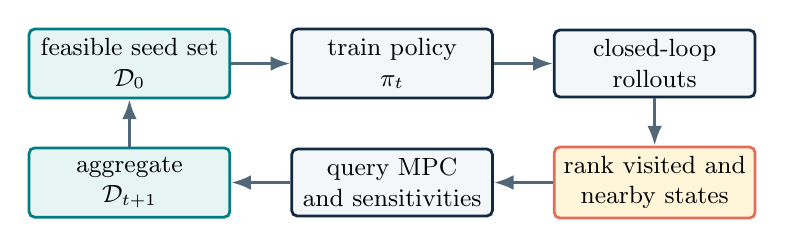
\begin{tikzpicture}[
  node distance=0.6cm and 0.75cm,
  every node/.style={font=\small,align=center},
  box/.style={draw=Ink,line width=1pt,rounded corners=2pt,minimum height=.85cm,minimum width=2.55cm,fill=Mist},
  arr/.style={-{Latex[length=2.5mm]},line width=1.1pt,Slate}
]
  \node[box,fill=Sky,draw=Teal] (seed) {feasible seed set\\$\D_0$};
  \node[box,right=of seed] (train) {train policy\\$\pi_t$};
  \node[box,right=of train] (roll) {closed-loop\\rollouts};
  \node[box,below=of roll,fill=PaleGold,draw=Coral] (query) {rank visited and\\nearby states};
  \node[box,left=of query] (expert) {query MPC\\and sensitivities};
  \node[box,left=of expert,fill=Sky,draw=Teal] (agg) {aggregate\\$\D_{t+1}$};
  \draw[arr] (seed)--(train);
  \draw[arr] (train)--(roll);
  \draw[arr] (roll)--(query);
  \draw[arr] (query)--(expert);
  \draw[arr] (expert)--(agg);
  \draw[arr] (agg)--(seed);
\end{tikzpicture}

\vspace{0.45cm}
\begin{columns}[T,onlytextwidth]
\column{0.48\textwidth}
\textbf{Why this loop matters}

The learned policy visits states that an expert-generated static dataset may not contain.

\column{0.48\textwidth}
\textbf{Why query selection still matters}

Labeling every visited state recovers DAgger-like robustness but can remain expensive. The acquisition rule decides which visits merit an OCP solve.
\end{columns}

\smallsource{Distribution shift and dataset aggregation: Ross, Gordon and Bagnell, AISTATS, 2011.}
\note{The key distinction from DAgger is that the expert is computationally expensive but differentiable and constrained. We can exploit both uncertainty and optimization structure to avoid querying every encountered state.}
\end{frame}

% -----------------------------------------------------------------------------
\begin{frame}{Adjacent literatures leave a useful intersection}
\scriptsize
\setlength{\tabcolsep}{4pt}
\renewcommand{\arraystretch}{1.35}
\begin{tabular}{>{\bfseries\color{Teal}}p{0.20\textwidth} p{0.27\textwidth} p{0.25\textwidth} p{0.20\textwidth}}
\toprule
Area & What it already contributes & Typical limitation for this problem & Opportunity \\
\midrule
Active learning & uncertainty and diversity based queries & pool-based labels, often without dynamics or feasibility & control-aware acquisition \\
Approximate MPC & fast learned policies and feasibility guarantees & datasets often treated as given & data design as part of controller design \\
Sensitivity methods & several local labels from one solve & local validity and active-set changes & adaptive neighborhoods and boundary detection \\
Imitation learning & correction of policy-induced distribution shift & expert queries can be assumed cheap & selective expert queries \\
Optimal design & principled criteria for information allocation & classical criteria may not reflect closed-loop risk & trajectory and constraint weighted design \\
\bottomrule
\end{tabular}

\vspace{0.38cm}
\normalsize
\colorbox{PaleGold}{\parbox{0.93\textwidth}{\centering
\textbf{Research gap:} integrate feasibility, parametric-program sensitivity, and policy-induced state distributions into one data-design problem.}}

\smallsource{Recent evidence includes prior-informed dynamics sampling (Miller, Thorpe and Topcu, 2024), active constraint learning (Qiu, Chiu and Chou, L4DC 2026), and feasible-set sampling for approximate MPC (Milios et al., 2026).}
\note{State the novelty claim carefully. Each ingredient exists. The underexplored part is their joint use for selecting expensive MPC labels according to closed-loop consequences.}
\end{frame}

% -----------------------------------------------------------------------------
\begin{frame}{Research questions for a mathematical collaboration}
\begin{enumerate}
  \item[\color{Teal}\bfseries Q1.] \textbf{Definition.} Which information functional connects a sampling distribution to closed-loop loss, feasibility, or stability?

  \item[\color{Teal}\bfseries Q2.] \textbf{Guarantees.} Under piecewise-smooth parametric policies, can prior-informed sampling improve label complexity over uniform feasible-set sampling?

  \item[\color{Teal}\bfseries Q3.] \textbf{Geometry.} How should a sampler allocate mass near active-set boundaries, disconnected feasible components, and thin safety-critical regions?

  \item[\color{Teal}\bfseries Q4.] \textbf{Adaptation.} Can one control bias and variance when $q_t$ depends on the current learned policy and on previous optimization outcomes?
\end{enumerate}

\vspace{0.25cm}
\begin{center}
\pill{Sky}{parametric optimization}\quad
\pill{PaleGold}{probability and statistics}\quad
\pill{Sky}{dynamical systems}\quad
\pill{PaleGold}{learning theory}
\end{center}
\note{These questions make the meeting collaborative. They are not requests for generic machine-learning help. They expose specific mathematical obstacles where department expertise can contribute.}
\end{frame}

% -----------------------------------------------------------------------------
\begin{frame}{A minimal first project}
\begin{columns}[T,onlytextwidth]
\column{0.61\textwidth}
\textbf{Benchmark}

A constrained nonlinear system such as cart-pole, followed by one switched-system or quadrupedal planning example.

\textbf{Four sampling baselines}
\begin{itemize}
  \item uniform box sampling with rejection,
  \item approximately uniform feasible-set sampling,
  \item active uncertainty sampling,
  \item the proposed structure-informed adaptive sampler.
\end{itemize}

\textbf{Fixed budget protocol}

Compare all methods for the same number of exact OCP solves, with identical network capacity and optimization settings.

\column{0.34\textwidth}
\textbf{Primary outcomes}
\begin{align*}
  &\text{closed-loop cost gap},\\
  &\text{constraint violation rate},\\
  &\text{feasible initial-state coverage},\\
  &\text{worst-case policy error},\\
  &\text{wall-clock data cost}.
\end{align*}

\vspace{0.15cm}
\colorbox{Sky}{\parbox{0.92\linewidth}{\centering First target: an empirical result plus one theorem in a tractable special case.}}
\end{columns}
\note{Keep the first project controlled. A linear or piecewise-affine case can support theory, while a nonlinear or switched example shows relevance to the user's research.}
\end{frame}

% -----------------------------------------------------------------------------
\begin{frame}{Why the problem has real research potential}
\begin{columns}[T,onlytextwidth]
\column{0.62\textwidth}
\small
\begin{itemize}
  \setlength{\itemsep}{0.12em}
  \item A 2026 paper still identifies feasible-set sampling as a major bottleneck for approximate MPC and reports an order-of-magnitude speedup for uniform sampling in the linear-polyhedral case.
  \item Sensitivity-based augmentation already shows that optimization derivatives reduce the number of exact expert evaluations.
  \item Recent active-learning theory explains why uncertainty and diversity can reduce label complexity, while control papers show gains from prior-informed exploration.
  \item Active constraint learning in 2026 outperforms random query selection in simulation and hardware experiments.
\end{itemize}

\column{0.33\textwidth}
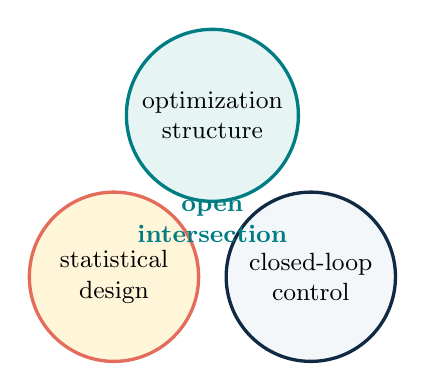
\begin{tikzpicture}[every node/.style={align=center,font=\small}]
  \node[draw=Teal,very thick,circle,minimum size=2.15cm,fill=Sky] (o) at (0,1.5) {optimization\\structure};
  \node[draw=Coral,very thick,circle,minimum size=2.15cm,fill=PaleGold] (s) at (-1.25,-.55) {statistical\\design};
  \node[draw=Ink,very thick,circle,minimum size=2.15cm,fill=Mist] (c) at (1.25,-.55) {closed-loop\\control};
  \node[font=\bfseries\small,Teal] at (0,.15) {open\\intersection};
\end{tikzpicture}
\end{columns}

\vspace{0.15cm}
\color{Slate}\scriptsize Assessment: the broad topic is established, but the control-specific formulation above is timely and sufficiently focused for a collaboration. Its novelty must be tested against the exact system class and guarantee sought.

\smallsource{Sources: Krishnamoorthy 2022, 2023; Bu et al., ICML 2024; Miller et al., 2024; Qiu et al., L4DC 2026; Milios et al., 2026.}
\note{This directly answers whether the idea has potential. Avoid claiming that nobody has combined these ingredients. Say that the intersection appears underexplored and that novelty depends on a precise theorem or algorithm.}
\end{frame}

% -----------------------------------------------------------------------------
\begin{frame}{A possible division of work}
\begin{columns}[T,onlytextwidth]
\column{0.48\textwidth}
{\color{Teal}\Large\bfseries What I bring}

\begin{itemize}
  \item constrained optimal control and NMPC,
  \item active-set exploration and feasible-set projection,
  \item switched and hybrid systems,
  \item robotic benchmarks and numerical implementation.
\end{itemize}

\column{0.48\textwidth}
{\color{Coral}\Large\bfseries Where collaboration helps}

\begin{itemize}
  \item probability measures and transport,
  \item optimal experimental design,
  \item sample-complexity and generalization analysis,
  \item geometry of parametric optimization.
\end{itemize}
\end{columns}

\vfill
\begin{center}
\colorbox{Ink}{\parbox{0.86\textwidth}{\centering\color{white}\large
Can we turn the structure of an optimal controller into a measurable reduction in the number of labels needed to learn it?}}
\end{center}
\note{End with a question that invites specific follow-up. The goal of the meeting is to identify one tractable theoretical angle and one professor interested in pursuing it.}
\end{frame}

% -----------------------------------------------------------------------------
\begin{frame}{Selected references}
\scriptsize
\begin{thebibliography}{9}
\setbeamertemplate{bibliography item}[text]

\bibitem{Hertneck2018}
M. Hertneck, J. K\"ohler, S. Trimpe, F. Allg\"ower.
\newblock Learning an Approximate Model Predictive Controller with Guarantees.
\newblock \emph{IEEE Control Systems Letters}, 2018. DOI: \href{https://doi.org/10.1109/LCSYS.2018.2843682}{10.1109/LCSYS.2018.2843682}.

\bibitem{Krish2022}
D. Krishnamoorthy.
\newblock A Sensitivity-based Data Augmentation Framework for Model Predictive Control Policy Approximation.
\newblock \emph{IEEE Transactions on Automatic Control}, 2022. DOI: \href{https://doi.org/10.1109/TAC.2021.3124983}{10.1109/TAC.2021.3124983}.

\bibitem{Krish2023}
D. Krishnamoorthy.
\newblock An Improved Data Augmentation Scheme for Model Predictive Control Policy Approximation.
\newblock \emph{IEEE Control Systems Letters}, 2023. DOI: \href{https://doi.org/10.1109/LCSYS.2023.3282383}{10.1109/LCSYS.2023.3282383}.

\bibitem{Ross2011}
S. Ross, G. Gordon, D. Bagnell.
\newblock A Reduction of Imitation Learning and Structured Prediction to No-Regret Online Learning.
\newblock \emph{AISTATS}, 2011. \href{https://proceedings.mlr.press/v15/ross11a.html}{PMLR 15:627--635}.

\bibitem{Pfrommer2022}
D. Pfrommer, T. Zhang, S. Tu, N. Matni.
\newblock TaSIL: Taylor Series Imitation Learning.
\newblock \emph{NeurIPS}, 2022. \href{https://proceedings.neurips.cc/paper_files/paper/2022/hash/7f10c3d66c3b7863a9cda255dcac5bb7-Abstract-Conference.html}{Paper page}.

\end{thebibliography}
\end{frame}

\begin{frame}
\frametitle{Selected references (continued)}
\scriptsize
\begin{thebibliography}{9}
\setbeamertemplate{bibliography item}[text]

\bibitem{Bu2024}
D. Bu, W. Huang, T. Suzuki, et al.
\newblock Provably Neural Active Learning Succeeds via Prioritizing Perplexing Samples.
\newblock \emph{ICML}, 2024. \href{https://proceedings.mlr.press/v235/bu24a.html}{PMLR 235:4642--4695}.

\bibitem{Miller2024}
K. S. Miller, A. J. Thorpe, U. Topcu.
\newblock Active Learning of Dynamics Using Prior Domain Knowledge in the Sampling Process.
\newblock arXiv:2403.17233, 2024. \href{https://arxiv.org/abs/2403.17233}{arXiv page}.

\bibitem{Qiu2026}
Z. Qiu, C.-Y. Chiu, G. Chou.
\newblock Active Constraint Learning in High Dimensions from Demonstrations.
\newblock \emph{L4DC}, 2026. \href{https://proceedings.mlr.press/v331/qiu26a.html}{PMLR 331:532--556}.

\bibitem{Milios2026}
E. Milios, F. Berkel, F. Gruber, M. N. Zeilinger, K. P. Wabersich.
\newblock Efficient Uniform Feasible-Set Sampling for Approximate Linear MPC.
\newblock arXiv:2604.09118v2, 2026. \href{https://arxiv.org/abs/2604.09118v2}{arXiv page}.

\end{thebibliography}

\vfill
\color{Slate}\tiny Literature checked online on 4 October 2026. The proposed research gap is an inference from the cited strands, not a claim of exhaustive novelty.
\end{frame}

% ============================== BACKUP =======================================
\appendix

\begin{frame}{Backup: differentiating the KKT system}
Let
\[
L(z,\nu,\lambda;x)=J(z;x)+\nu^\top c(z;x)+\lambda^\top g(z;x).
\]
For a fixed active set $\mathcal A$, the sensitivity solves
\[
\underbrace{
\begin{bmatrix}
\nabla^2_{zz}L & c_z^\top & g_{\mathcal A,z}^\top\\
c_z & 0 & 0\\
g_{\mathcal A,z} & 0 & 0
\end{bmatrix}}_{F_y}
\begin{bmatrix}
D_xz^\star\\D_x\nu^\star\\D_x\lambda^\star_{\mathcal A}
\end{bmatrix}
=-
\underbrace{
\begin{bmatrix}
\nabla^2_{zx}L\\c_x\\g_{\mathcal A,x}
\end{bmatrix}}_{F_x}.
\]

Local differentiability requires regularity conditions such as LICQ, strict complementarity, and a suitable second-order condition. Near active-set changes, generalized derivatives or predictor-corrector tracking may be more appropriate.
\note{Use this slide only if the audience asks where policy sensitivities come from. It also explains why active-set boundaries are statistically important and analytically difficult.}
\end{frame}

\begin{frame}{Backup: success criteria and ablations}
\renewcommand{\arraystretch}{1.4}
\begin{tabular}{>{\bfseries\color{Teal}}p{0.25\textwidth} p{0.31\textwidth} p{0.34\textwidth}}
\toprule
Question & Experiment & Desired evidence \\
\midrule
Does structure help? & remove sensitivity, boundary, or occupancy terms one at a time & consistent degradation under a fixed label budget \\
Does it generalize? & test shifted initial-state and reference distributions & controlled risk under moderate distribution shift \\
Does it remain safe? & stress states near constraints and feasible-set boundary & lower violation rate than uncertainty-only sampling \\
Does it scale? & increase state dimension, horizon, and number of modes & favorable solver calls and wall-clock scaling \\
Is the gain real? & repeat over seeds and report confidence intervals & statistically resolved improvement \\
\bottomrule
\end{tabular}
\end{frame}

\end{document}
